\documentclass[aspectratio=169,12pt]{beamer}
\usetheme{Madrid}
\usecolortheme{dolphin}
\usefonttheme{professionalfonts}
\setbeamertemplate{navigation symbols}{}
\setbeamertemplate{footline}{}

\usepackage[T1]{fontenc}
\usepackage[utf8]{inputenc}
\usepackage{graphicx}
\usepackage{amsmath,amssymb}
\usepackage{hyperref}
\usepackage{siunitx}
\usepackage{physics}
\usepackage{braket}
\usepackage{tikz}
\usetikzlibrary{calc}

\title[Chapter 5]{Chapitre 5: Mesure, projection, probabilité du résultat et bases arbitraires}
\author{JAMOTTE Maxime, SCHOONEN Cédric}
\institute{Digital Learning Hub}
\date{}

\newcommand{\projectionfiguresimple}{%
  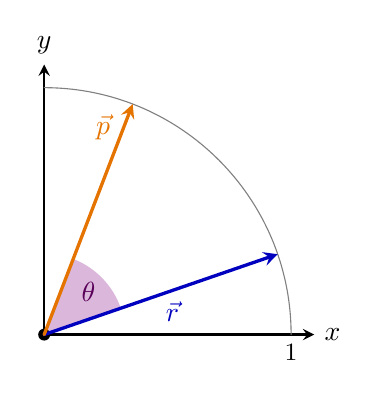
\begin{tikzpicture}[scale=0.98, line cap=round, line join=round, >=stealth]
    \coordinate (O) at (0,0);
    \coordinate (X) at (3.5,0);
    \coordinate (Y) at (0,3.5);
    \coordinate (R) at ({3.2*cos(19)},{3.2*sin(19)});
    \coordinate (P) at ({3.2*cos(69)},{3.2*sin(69)});

    \fill[violet!28] ({1.05*cos(19)},{1.05*sin(19)})
      arc[start angle=19, end angle=69, radius=1.05] -- (O) -- cycle;

    \draw[->, thick] (O) -- (X) node[right] {$x$};
    \draw[->, thick] (O) -- (Y) node[above] {$y$};
    \fill (O) circle (2.2pt);
    \draw[gray] (3.2,0) arc[start angle=0, end angle=90, radius=3.2];
    \node[below] at (3.2,0) {\small 1};

    \draw[->, very thick, blue!75!black] (O) -- (R) node[pos= 0.55, below] {$\vec r$};
    \draw[->, very thick, orange!90!black] (O) -- (P)
      node[pos=0.9, left=1pt, text=orange!90!black] {$\vec p$};

    \node[violet!70!black] at ({0.8*cos(44)},{0.8*sin(44)}) {$\theta$};
  \end{tikzpicture}%
}

\newcommand{\projectionfigureMQ}{%
  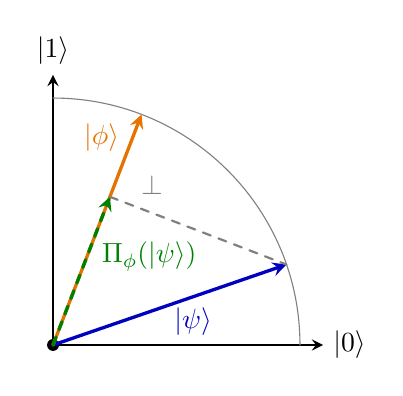
\begin{tikzpicture}[scale=0.98, line cap=round, line join=round, >=stealth]
    \coordinate (O) at (0,0);
    \coordinate (X) at (3.5,0);
    \coordinate (Y) at (0,3.5);
    \coordinate (R) at ({3.2*cos(19)},{3.2*sin(19)});
    \coordinate (P) at ({3.2*cos(69)},{3.2*sin(69)});
    \coordinate (Proj) at ({3.2*cos(50)*cos(69)},{3.2*cos(50)*sin(69)});

    \draw[->, thick] (O) -- (X) node[right] {$\ket 0$};
    \draw[->, thick] (O) -- (Y) node[above] {$\ket 1$};
    \fill (O) circle (2.2pt);
    \draw[gray] (3.2,0) arc[start angle=0, end angle=90, radius=3.2];
    

    \draw[->, very thick, blue!75!black] (O) -- (R) node[pos= 0.6, below] {$\ket \psi$};
    
    \draw[->, very thick, orange!90!black] (O) -- (P)
      node[pos=0.9, left=1pt, text=orange!90!black] {$\ket \phi$};
    \draw[dashed,->, very thick, green!50!black] (O) -- (Proj);
    \draw[dashed, thick, gray] (Proj) -- (R);

    \node[text=green!50!black] at ({1.65*cos(44)},{1.65*sin(44)}) {$\ {\Pi}_{\phi}(\ket \psi)$};
    \node[gray] at ($(Proj)!0.5!(R)+(-0.6,0.6)$) {$\perp$};
  \end{tikzpicture}%
}

\newcommand{\projectionfigure}{%
  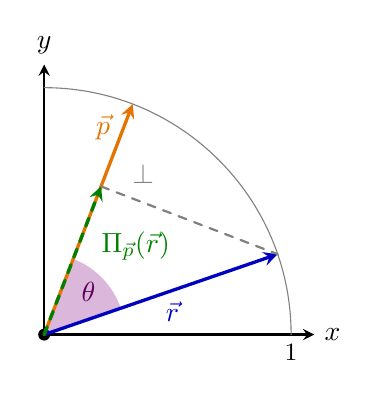
\begin{tikzpicture}[scale=0.98, line cap=round, line join=round, >=stealth]
    \coordinate (O) at (0,0);
    \coordinate (X) at (3.5,0);
    \coordinate (Y) at (0,3.5);
    \coordinate (R) at ({3.2*cos(19)},{3.2*sin(19)});
    \coordinate (P) at ({3.2*cos(69)},{3.2*sin(69)});
    \coordinate (Proj) at ({3.2*cos(50)*cos(69)},{3.2*cos(50)*sin(69)});

    \fill[violet!28] ({1.05*cos(19)},{1.05*sin(19)})
      arc[start angle=19, end angle=69, radius=1.05] -- (O) -- cycle;

    \draw[->, thick] (O) -- (X) node[right] {$x$};
    \draw[->, thick] (O) -- (Y) node[above] {$y$};
    \fill (O) circle (2.2pt);
    \draw[gray] (3.2,0) arc[start angle=0, end angle=90, radius=3.2];
    \node[below] at (3.2,0) {\small 1};
    \draw[->, very thick, blue!75!black] (O) -- (R) node[pos= 0.55, below] {$\vec r$};
    
    \draw[->, very thick, orange!90!black] (O) -- (P)
      node[pos=0.9, left=1pt, text=orange!90!black] {$\vec p$};
    \draw[dashed,->, very thick, green!50!black] (O) -- (Proj);
    \draw[dashed, thick, gray] (Proj) -- (R);

    \node[text=green!50!black] at ({1.65*cos(44)},{1.65*sin(44)}) {${\Pi}_{\vec p}(\vec r)$};
    \node[gray] at ($(Proj)!0.5!(R)+(-0.6,0.6)$) {$\perp$};
    \node[violet!70!black] at ({0.8*cos(44)},{0.8*sin(44)}) {$\theta$};
  \end{tikzpicture}%
}

%==============================================
%==============================================

\begin{document}

\begin{frame}
  \titlepage
\end{frame}

\begin{frame}{Objectifs du chapitre 5}
    \begin{itemize}
        \item Définir la mesure en mécanique quantique \\~\\
        \item Relier mesure, projection, produit scalaire, vecteurs propres et valeurs propres\\~\\
        \item Probabilité de mesure\\~\\
        \item Mesurer dans d'autres bases\\~\\
        \item Mesurer avec QISKIT
    \end{itemize}
\end{frame}

\begin{frame}{Mesurer un qubit}
  \begin{itemize}[<+->]
    \setlength{\itemsep}{0.6em}
    \item État général d'un qubit: $\ket{\psi} = \alpha \ket 0 + \beta \ket 1$.
    \\~\\
    \item Mesurer un qubit donne \textbf{un seul résultat}: $\ket{0}$ ou $\ket{1}$ (dans la base computationnelle).
    \\~\\
    \item Les probabilités sont données par le \textbf{carré des coefficients}:
    $$P(\ket 0) = |\alpha|^2, \qquad P(\ket 1) = |\beta|^2$$
    \item Après la mesure, l'état est \textbf{projeté} sur le résultat obtenu ($\ket{0}$ ou $\ket{1}$).
  \end{itemize}
\end{frame}

\begin{frame}{Projection}
  \begin{columns}[T]
    \begin{column}{0.6\textwidth}
      \begin{itemize}
        \setlength{\itemsep}{0.6em}
        \item Projection du vecteur $\vec r$ sur $\vec p$: $$\Pi_{\vec p}(\vec r) = (\vec r \cdot \vec p)\ \vec p$$
      \end{itemize}
    \end{column}
    \begin{column}{0.35\textwidth}
      \centering
      \projectionfiguresimple
    \end{column}
  \end{columns}
\end{frame}

\begin{frame}{Projection}
  \begin{columns}[T]
    \begin{column}{0.6\textwidth}
      \begin{itemize}
        \setlength{\itemsep}{0.6em}
        \item Projection du vecteur $\vec r$ sur $\vec p$: $$\Pi_{\vec p}(\vec r) = (\vec r \cdot \vec p)\ \vec p$$
      \end{itemize}
    \end{column}
    \begin{column}{0.35\textwidth}
      \centering
      \projectionfigure
    \end{column}
  \end{columns}
\end{frame}

\begin{frame}{Projection et produit scalaire}
  \begin{columns}[T]
    \begin{column}{0.6\textwidth}
      \begin{itemize}
        \setlength{\itemsep}{0.6em}
        \item Projection du vecteur $\vec r$ sur $\vec p$: $$\Pi_{\vec p}(\vec r) = (\vec r \cdot \vec p)\ \vec p$$
        \item Produit scalaire:
        $$\vec r \cdot \vec p = \begin{pmatrix} a & b \end{pmatrix} \begin{pmatrix} c \\ d \end{pmatrix} = ac+bd$$
        \item Lien avec l'angle: $\vec r \cdot \vec p = \norm{\vec r}\norm{\vec p}\cos(\theta)$
        %\item Produit scalaire entre deux états $\ket{\phi}$ et $\ket \psi$: $\braket{\phi|\psi}$.
      \end{itemize}
    \end{column}
    \begin{column}{0.35\textwidth}
      \centering
      \projectionfigure
    \end{column}
  \end{columns}
\end{frame}

\begin{frame}{Projection en mécanique quantique: notation ket-bra}
  \begin{itemize}[<+->]
    \setlength{\itemsep}{0.6em}
    \item L'état d'un qubit sous forme $\ket \psi$ s'écrit $\begin{pmatrix}
    \alpha\\ \beta \end{pmatrix}$ \\~\\
    \item L'état d'un qubit sous forme $\bra \psi$ s'écrit $\begin{pmatrix}
    \alpha \ \beta \end{pmatrix}$ (si $\alpha, \beta \in \mathbb R$) \\~\\
    \item Projecteur sur l'état $\ket \psi$: $$\Pi_\psi^{} = \ket \psi \bra \psi$$ 
  \end{itemize}
\end{frame}

\begin{frame}{Projecteurs en notation matricielle}
  \begin{itemize}[<+->]
    \setlength{\itemsep}{0.6em}
    \item $\Pi_\psi^{} = \ket \psi \bra \psi = (\alpha \  \beta) \begin{pmatrix}
    \alpha \\ \beta
    \end{pmatrix} = \begin{pmatrix}
      \alpha^2 & \alpha \beta\\
      \alpha \beta & \beta^2
    \end{pmatrix}$\\~\\
    \item Les projecteurs $\Pi_0$ et $\Pi_1$ s'écrivent aussi comme des matrices $2\times 2$:
    $$\Pi_0 = \ket{0}\bra{0} =
      \begin{pmatrix}1\\0\end{pmatrix}\begin{pmatrix}1 & 0\end{pmatrix}
      = \begin{pmatrix}1 & 0\\0 & 0\end{pmatrix}$$
    $$\Pi_1 = \ket{1}\bra{1} =
      \begin{pmatrix}0\\1\end{pmatrix}\begin{pmatrix}0 & 1\end{pmatrix}
      = \begin{pmatrix}0 & 0\\0 & 1\end{pmatrix}$$
    %\item On vérifie la relation de complétude:    $\Pi_0 + \Pi_1 = \begin{pmatrix}1 & 0\\0 & 1\end{pmatrix} = I$ (matrice identité).
    %\item La probabilité de mesurer $\ket{0}$ s'écrit: $P(0) = \bra{\psi}\Pi_0\ket{\psi} = |\alpha|^2$.
  \end{itemize}
\end{frame}

\begin{frame}{Projection et produit scalaire en mécanique quantique}
  \begin{columns}[T]
    \begin{column}{0.6\textwidth}
      \begin{itemize}
        \setlength{\itemsep}{0.6em}
        \item Projecteur sur l'état $\ket{\phi}$: $\Pi_\phi^{} = \ket{\phi}\bra{\phi}$\\~\\
        \item Projection de $\ket \psi$ sur l'état $\ket{\phi}$: $$ \Pi_\phi^{}(\ket{\psi}) =  \ket{\phi}\braket{\phi|\psi}$$
        \item Produit scalaire entre deux états $\ket{\phi}$ et $\ket \psi$: $\braket{\phi|\psi}$.\\~\\
      \end{itemize}
    \end{column}
    \begin{column}{0.35\textwidth}
      \centering
      \projectionfigureMQ
    \end{column}
  \end{columns}
\end{frame}

\begin{frame}{Produit scalaire en mécanique quantique}
  \begin{columns}[T]
    \begin{column}{0.6\textwidth}
      \begin{itemize}
        \setlength{\itemsep}{0.6em}
        \item Produit scalaire entre deux états $\ket{\phi}$ et $\ket \psi$: $$\braket{\phi|\psi}$$\\~\\
         \item Conventions: $\braket{0|0} = 1$, $\braket{1|1} = 1$ et $\braket{0|1} = 0$ (orthogonaux).
      \end{itemize}
    \end{column}
    \begin{column}{0.35\textwidth}
      \centering
      \projectionfigureMQ
    \end{column}
  \end{columns}
\end{frame}

\begin{frame}{Projection, produit scalaire et probabilité de mesure}
  \begin{itemize}[<+->]
    \setlength{\itemsep}{0.6em}
    \item Mesurer $\ket \psi$ le projette dans l'état $\ket 0$ ou $\ket 1$: 
    $$\Pi_0^{} \ket \psi = \alpha \ket 0, \quad \Pi_1^{} \ket \psi = \beta \ket 1$$
    \item La probabilité de mesurer $\ket{0}$ ou $\ket 1$ s'écrit comme le produit scalaire de $\ket \psi$ avec sa projection sur l'état $\ket 0$ ou $\ket 1$:
    $$P(0) = \bra{\psi}\Pi_0\ket{\psi} = |\alpha|^2$$
    $$P(1) = \bra{\psi}\Pi_1\ket{\psi} = |\beta|^2$$
  \end{itemize}
\end{frame}

% ============================================================
\section{Reproductibilité de la mesure}
% ============================================================

\begin{frame}{Reproductibilité de la mesure: $\Pi^2 = \Pi$}
  \begin{itemize}[<+->]
    \setlength{\itemsep}{0.8em}
    \item La mesure \textbf{projette} l'état quantique sur $\ket{0}$ ou $\ket{1}$
     selon les probabilités $P(\ket 0)$ et $P(\ket 1)$.\\~\\
    \item Si on mesure à nouveau, on retrouve le même résultat: la mesure est reproductible.\\~\\
    \item Mathématiquement: $\Pi^2 = \Pi$, c'est pourquoi la mesure est une projection.\\~\\
    \item L'état $\ket 0$ reste intact sous l'action de $\Pi_0^{}$: $\Pi_0^{} \ket 0 = \ket 0$\\~\\ 
    \item $\ket 0$ est un \textbf{état propre} du projecteur $\Pi_0^{}$.
  \end{itemize}
\end{frame}

\begin{frame}{Valeurs propres et vecteurs propres}
  \begin{itemize}[<+->]
    \setlength{\itemsep}{0.6em}
    \item On dit aussi que le vecteu représentant l'état $\ket 0$ est un vecteur propre de la matrice représentant le projecteur $\Pi_0^{}$\\~\\
    \item Autre exemple d'un produit matrice-vecteur:   
    $$ \begin{pmatrix} 2 & 1 \\ 2 & 3 \end{pmatrix} \begin{pmatrix} -1 \\ 1 \end{pmatrix} = \begin{pmatrix} -1 \\ 1 \end{pmatrix},$$
    et 
    $$ \begin{pmatrix} 2 & 1 \\ 2 & 3 \end{pmatrix} \begin{pmatrix} 1 \\ 2 \end{pmatrix} = \begin{pmatrix} 4 \\ 8 \end{pmatrix} = 4 \begin{pmatrix} 1 \\ 2 \end{pmatrix},$$~\\
    \item Multiplier ce vecteur par cette matrice redonne le même vecteur multiplié par un nombre.
    \item On nomme ce vecteur "\textbf{vecteur propre}" et ce nombre "\textbf{valeur propre}".
  \end{itemize}
\end{frame}

\begin{frame}{Les états $\ket 0, \ket 1$ sont des vecteurs propres d'une observable}
  \begin{itemize}[<+->]
    \setlength{\itemsep}{0.6em}
    \item Les grandeurs mesurables sont représentées par des matrices appelées \textit{observables}.
    \item \textbf{Mesurer} une quantité physique revient à mesurer l'une de ses \textbf{valeurs propres}.
    \item Les états $\ket{0}$ et $\ket{1}$ sont les vecteurs propres de l'observable $Z$
     (base computationnelle):
    $$Z\ket{0} = +\ket{0}, \qquad Z\ket{1} = -\ket{1}$$
    \item La nature physique de la valeur propre (énergie, spin,...) dépend de la plateforme (voir plus tard).
    \item \textbf{Postulat}: mesurer = projeter le vecteur du qubit sur le vecteur propre associé à la
     valeur propre de l'observable mesurée.
  \end{itemize}
\end{frame}

% ============================================================
\section{Autres bases et observables}
% ============================================================

\begin{frame}{Projection sur des vecteurs arbitraires}
  \begin{itemize}[<+->]
    \setlength{\itemsep}{0.8em}
    \item On peut mesurer dans d'autres bases que la base computationnelle $\{\ket{0}, \ket{1}\}$.\\~\\
    \item Par exemple, la base $\{\ket{+}, \ket{-}\}$ avec:
    $$\ket{+} = \frac{\ket{0}+\ket{1}}{\sqrt{2}}, \qquad \ket{-} = \frac{\ket{0}-\ket{1}}{\sqrt{2}}$$
    \item Les vecteurs $\ket{+}$ et $\ket{-}$ sont les vecteurs propres de l'observable $X$:
    $$X\ket{+} = (+1)\ket{+}, \qquad X\ket{-} = (-1)\ket{-}$$
    \item On peut ainsi définir des projecteurs et probabilités de mesure dans cette base.
  \end{itemize}
\end{frame}

\end{document}
